% Templates
\begin{comment}

\begin{figure}[H]
	\centering
	\includegraphics[width=0.7\textwidth]{tyristor/}
	\caption{}
	\label{fig:}
\end{figure}

\vspace{0.5cm} % Add space after the solution

\begin{enumerate}[label=\roman*)]
	\item 
	\item
\end{enumerate}

\end{comment}

\begin{question}[name=Spørsmål, topic=tyristor]
	En tyristor kan brukes som bryter for å koble inn og ut en likestrøm gjennom en magnetspole. Styrestrømmen til tyristoren kommer fra en impulsbryter. Hvordan skal strømmen gjennom tyristoren slåes av?
\end{question}

\vspace{0.5cm} % Add space after the solution

\begin{solution}[name=Løsningsforslag]
	Ved å bryte hovedstrømmen
\end{solution}

\vspace{0.5cm} % Add space after the solution

\begin{question}[name=Spørsmål, topic=tyristor]
Hva er forskjellen mellom en tyristor og en transistor?
\end{question}

\vspace{0.5cm} % Add space after the solution

\begin{solution}[name=Løsningsforslag]
En tyristor kan kun ha diskrete tilstander, det vil si enten på eller av, mens en transistor kan operere kontinuerlig i mellomliggende tilstander og brukes til å regulere forsterkningen.
\end{solution}


\begin{question}[name=Spørsmål, topic=tyristor]
	
\begin{figure}[H]
	\centering
	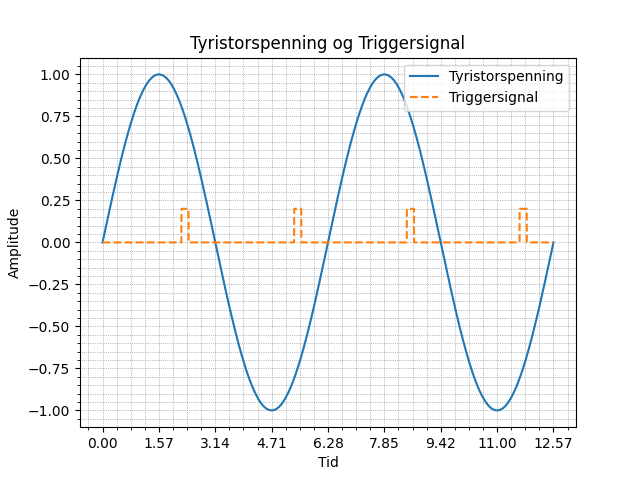
\includegraphics[width=0.9\textwidth]{tyristor/plot/tyristor2.png}
	\caption{Tyristor med triggersignal}
	\label{fig:tyrTriggplot}
\end{figure}
\end{question}

\vspace{0.5cm} % Add space after the solution

\begin{solution}[name=Løsningsforslag]
I Figur \ref{fig:tyrTriggplotSOL} kan man se hvordan tyristoren starter å lede ved positiv halvperode og når den får triggersignal. Tyristoren slutter å lede ved nullgjennomgangen.

\begin{figure}[H]
	\centering
	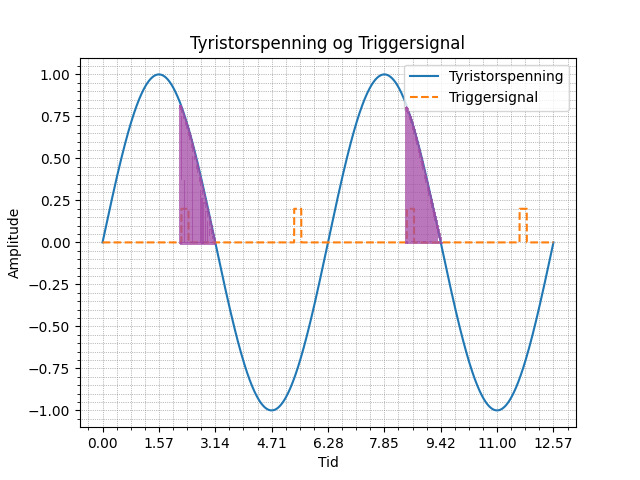
\includegraphics[width=0.9\textwidth]{tyristor/plot/tyristor2SOL.png}
	\caption{Tyristor med triggersignal}
	\label{fig:tyrTriggplotSOL}
\end{figure}

\end{solution}



% ------------------- TRIAC -------------------

\begin{question}[name=Spørsmål, topic=tyristor]
Beskriv funksjon til TRIAC koblingen i kretsen som vist i Figur \ref{fig:triPush}.
\begin{figure}[H]
	\centering
	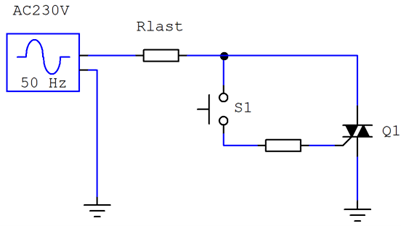
\includegraphics[width=0.7\textwidth]{tyristor/figurer/tricBasic.png}
	\caption{Triac krets med impulsbryter}
	\label{fig:triPush}
\end{figure}
\end{question}

\vspace{0.5cm} % Add space after the solution

\begin{solution}[name=Løsningsforslag]
TRIAC koblingen sørger for at man kan styre en større strøm ved hjelp av signal som trekker en mindre strøm.

TRIAC koblingen sørger for at kretsen blir brutt ved nullgjennomgangen som er spesielt fordelaktig når man bryter induktive kretser som potensielt vil kunne generere høy spenning og skade utstyret. Dette oppstår siden spenningen over en induktans er proporsjonal til endringsraten av strømmen gjennom induktansen som vist i Formel \ref{eq:strømInd}.

\begin{equation}
	\label{eq:strømInd}
	U_{ind}=L \cdot \frac{dI_{ind}}{dt}
\end{equation}

\end{solution}



% ------------------- DIAC -------------------


